\chapter{Introduction}

\section{Présentation du sujet}
Le module \emph{Initiation à la recherche} du 2\up{nd} semestre du master \textsc{ALMA} propose une initiation au métier de chercheur en informatique. Dans le cadre de ce module notre binôme a choisi le sujet : \emph{Conception et réalisation d’un logiciel interactif de visualisation de pavages 2D/3D}. Ce sujet à la particularité d'être la reprise d'un projet de stage. Ce stage, effectué au cours de l'été 2011 par un des membres du binôme, avait pour objectif initial la conception et la réalisation d'un outil de visualisation des calculs en sortie du logiciel \realpaver (\cf{} Section \ref{realp}), développé au sein de l'équipe d'accueil.% Le développement de ce stage a suivit le modèle du cycle en V.

% décrit par la figure \ref{fig:vcycle}.
% \begin{figure}[htbp]
% \centering
% 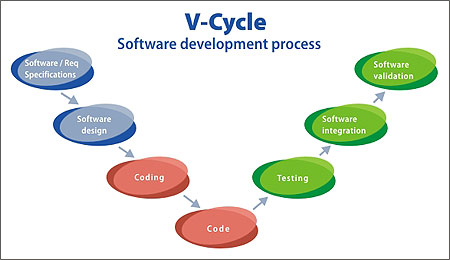
\includegraphics[scale=1]{img/vcycle}
% \caption{Cycle en V}
% \label{fig:vcycle}
% \end{figure}
% \clearpage
\paragraph{}
Au terme des deux mois de ce stage, le travail accompli fut le suivant :
\begin{enumerate}
\item 
Rédaction du cahier des charges (\cf{} Annexe \ref{sec:cac})
\item
Rédaction du document de spécification (\cf{} Annexe \ref{sec:spe}).
\end{enumerate} 



%exlpliquer ce que fait le logiciel (entrée et sortie),projection des dimensions notions fe,être de visualisation( ce n'est quune partie du pavage ... )  
\section{Équipe d'accueil}
L'équipe Optimisation globale, optimisation multi-objectifs\cite{opti} (\textsc{OPTI}) du laboratoire \textsc{LINA}\cite{lina} travaille principalement sur des méthodes visant à la résolution efficace de problèmes d’optimisation complexes.  

\section{Déroulement du projet}
Au cours des premières semaines, C.\textsc{Jermann} nous a proposé d'étudier de manière générale les sujets de l'équipe \textsc{OPTI}. Un bref bilan de cette étude est proposé dans le chapitre \ref{chap:doc}. En parallèle, nous avons manipulé quelques outils ad-hoc tel que \emph{gnuplot} \cite{gnu}, utilisés jusqu'à présent par l'équipe \textsc{OPTI} pour représenter les valuations calculées par \realpaver. Par la suite nous avons pris (ou repris) connaissance du cahier des charges et du document de spécifications, en apportant certaines corrections à ce dernier. 

\paragraph{}Une problématique est apparue quant à l'axe d'étude à choisir pour le déroulement du projet. En effet une des caractéristiques principale de l'outil à concevoir, est de manipuler un nombre potentiellement très grand de données (\cf{} Chapitre \ref{chap:con}). Nos alternatives étaient alors les suivantes : 
\begin{enumerate}
\item
Étudier les différents algorithmes et structures de données nécessaires à l'outil.
\item
Entamer directement la conception de l'outil (choix de design pattern, IHM, \dots).
\end{enumerate} 
Ce second choix impliquait la possibilité au terme de l'année, de proposer un résultat \og matériel \fg{}. En effet le document de spécifications étant très concis, nous aurions pu rapidement produire du code en le suivant à la lettre. Cependant cette démarche ne répondait pas aux objectifs de découverte du module d'\emph{Initiation à la recherche}. De plus, passer outre cette étude de structures et d'algorithmes, aurait rapidement entraîné la conception dans une impasse. Nous avons donc choisi la seconde alternative. Notre contribution à cette étude est résumée dans le chapitre \ref{chap:con} de ce document.


\section{Caractéristiques de l'outil}
Nous rappellerons dans cette section quelques notions propres à l'outils et indispensables à la compréhension de cette étude.  
\begin{description}
\item[Données en entrée] Un format spécifique à l'outil est défini dans le document de spécifications(\cf{} Annexe \ref{sec:spe}).
 \item[Fenêtre de visualisation] Il s'agit de la partie du pavage visible à l'écran à un instant~t. Selon le cahier des charges, l'utilisateur peut \og naviguer\fg{} dans l'environnement contenant le pavage. La gestion de la fenêtre de visualisation est l'une des problématiques abordées dans cette étude (\cf{} Section \ref{sec:vis}).
\item[Dimensions visualisées] L'intitulé du sujet d'étude précise que l'outil doit permettre une visualisation de deux ou trois dimensions. Cependant \realpaver{} est en mesure de calculer des problèmes à $n$ dimensions. L'utilisateur doit donc préciser les deux ou trois variables sur lesquelles seront effectuées la projection du pavage.  
\item[Filtre] Le cahier des charges demande la possibilité d'appliquer des filtres sur le pavage. Il s'agit d'effectuer une classification des boîtes déterminée par l'utilisateur (\cf{} Annexe \ref{sec:spe} section 1.2, 5\up{ème} point). Une telle opération sur le pavage va nécessiter de nombreuses opérations (accès aux caractéristiques d'une boîte, tris,\dots). La mise en œuvre de ces opérations est l'une des problématiques principale de la conception.    
\item[Données en sortie] Une sauvegarde du pavage visualisé est demandé par le cahier des charges. Il s'agit pour l'outil d'une simple \og sauvegarde \fg{} utilisant le même format que le fichier d'entrée. La création d'images à partir de l'écran de visualisation est aussi demandée.(\cf{} Annexe \ref{sec:spe})
\end{description}
